\documentclass[a4paper,12pt]{report}
\usepackage{algorithmic}
\usepackage[linesnumbered,ruled,vlined]{algorithm2e}
\SetKwRepeat{Do}{do}{while}
\usepackage[margin=2cm]{geometry}
\usepackage[utf8]{inputenc}
\usepackage{listings} 
\usepackage{graphicx} 
\usepackage{color}
\usepackage{xcolor}
\usepackage{hyperref}
%\usepackage{mdframed}

\newcommand{\currentdata}{ 1 February 2017}
\newtheorem{example}{Example}

\begin{document}
\vspace{-5cm}
\begin{center}
Department of Computer Science\\
Technical University of Cluj-Napoca\\

\includegraphics[width=10cm]{fig/footer}
\end{center}
\vspace{1cm}
%\maketitle
\begin{center}
\begin{Large}
 %\textbf{Introduction to Artificial Intelligence}\\
\textbf{Inductive learning - PFOIL}\\
\end{Large}
\textit{Laboratory activity 2016-2017}\\
\vspace{3cm}
Project title: ....\\
Tool: GNU Common Lisp\\
\vspace{1.5cm}
Name:Tomoiagă Andreea Ioana\\
Group:30235\\
Email:tandrioana@yahoo.com\\
\vspace{6cm}
Assoc. Prof. dr. eng. Adrian Groza\\
Adrian.Groza@cs.utcluj.ro\\
\vspace{1cm}

\includegraphics[width=10cm]{fig/footer}
\end{center}

\tableofcontents

%\chapter{Laboratory works}

\chapter{AI projects and tools ($W_1$)}

\section{Exercises}
\begin{enumerate}
 \item Compile the \texttt{is.tex} file in order to start writing your notes. 
Recall that this documentation is also a \textit{support for you}, during the design and implementation of you ideas. 
Make an habit in writing down your ideas from the first week in a professional manner.
\item Identify 3 Web resources with ideas on student AI projects.
\item Think at one of your hobbies. Would be possible to develop something on that line?
\item Identify a media source for AI-news. Investigate interesting ideas in that news. 
Do the AI-technologies behind these ideas appear in the AIMA book?
\item Identify AI journals in Science Direct and Springer Verlag. Browse some abstracts from these journals.
\item Identify an AI competition. Consider making a team of 2-3 students to participate at that competition.
\item Imagine that you are the founder of a start-up. What kind of innovative project would be feasible for you company? 
\item Write a short list (3 to 5) of possible projects for this lab. Be ambitios. 
\item Display network information for your workstation.
\item Connect via \texttt{ssh} to another workstation. 
\end{enumerate}

\fbox{\begin{minipage}{16cm}
Solution to exercise 2\\  
Trei surse cu idei de proiecte pentru studenti in domeniul inteligentei artifiala sunt:
\begin{itemize}
\item \href{http://nevonprojects.com/artificial-intelligence-projects/}{NevonProjects}
\item \href{https://www.crazyengineers.com/threads/artificial-intelligence-project-ideas-topics-for-engineering-students.58508/}{CrazyEngineers}
\item \href{https://www.quora.com/What-kind-of-final-year-projects-can-be-done-on-Artificial-Intelligence}{Final project ideas}
\end{itemize}   
\end{minipage}}
\vspace{0.5cm}

\fbox{\begin{minipage}{16cm}
Solution to exercise 3 \\
In lista hobby-urilor mele se regaseste placerea de a calatori, de a realiza drumetii. Folosind algoritmi din aria Inductive learning este posibila realizarea unui proiect bazat pe hobby-ul mentionat anterior. Acest proiect ar presupune implementarea unui sistem care sa decida daca calatoria intr-un loc specificat este una avantajoasa in functie de anumiti factori externi( buget, conditii de cazare, vreme, recomandari, atractiile turistice, etc).
\end{minipage}}
\vspace{0.5cm}

\fbox{\begin{minipage}{16cm}
Solution to exercise 4\\
AcListant este un prototip de sistem ajutator pentru controlul traficului aerian. Acest sistem se foloseste de algoritmi de speech recognition, algoritmi utilizati in identificarea comenzilor esentiale comunicate de un controller de trafic de zbor(altitudine, longitudine). Prototipul foloseste de asemenea o verificare a realitatii prin preluarea informatiilor curente ale radarului si interpretarea acestora in posibile propozitii cu informatii despre traficul aerian.\\
Sistemul se foloseste de algoritmi de speech recognition, tehnica prezenta si discutata si in AIMA.\\
Sursa catre stirea descrisa este urmatoarea: \href{https://www.sciencedaily.com/releases/2017/03/170308114851.htm}{AcListant}    
\end{minipage}}
\vspace{0.5cm}

\fbox{\begin{minipage}{16cm}
Solution to exercise 5\\
AI Journal abstracte:
\begin{itemize}
\item \href{http://www.sciencedirect.com/science/article/pii/S0004370217300048}{Human–computer negotiation}
\item \href{http://www.sciencedirect.com/science/article/pii/S0004370217300243}{Social ridesharing}
\item \href{https://link.springer.com/article/10.1007/s10489-014-0629-7}{Speech recognition}
\end{itemize} 
\end{minipage}}
\vspace{0.5cm}

\fbox{\begin{minipage}{16cm}
Solution to exercise 6 \\
O competitie interesanta si provocatoare de pe site-ul Kaggle este \href{https://www.kaggle.com/c/youtube8m}{Clasificarea video-urilor de pe Youtube}  
\end{minipage}}
\vspace{0.5cm}

\fbox{\begin{minipage}{16cm}
Solution to exercise 7 \\  
Tot mai multe proiecte actuale se bazeaza pe monitorizarea traficului, intrucat in ziua de azi orele de varf presupun o supraaglomeratie. Traficul este o problema prezenta in viata de zi cu zi. De asemenea, o alta problema cu care societatea se confrunta este supraaglomerarea localurilor. Astfel, consider ca un sistem de monitorizare a locurilor posibile de petrecere a timpului liber este un proiect realizabil si inovativ. Sistemul ar presupune determinarea locului prin algoritmi de inteligenta artificiala care ar tine cont de activitatea dorita, de locatia actuala a utilizatorului si de preferinte ale acestuia.   
\end{minipage}}
\vspace{0.5cm}

\fbox{\begin{minipage}{16cm}
Solution to exercise 8 \\
Posibile proiecte utilizand Inductive learning:
\begin{itemize}
\item Sistem utilizat pentru diagnosticul medical de leucemie.
\item Sistem utilizat pentru determinarea traseului optim la ore de varf.
\item Sistem utilizat pentru determinarea necesitatii trimiterii unui laptop in service in functie de  problemele hardware/software ale acestuia.
\item Sistem utilizat pentru sesizarea posibilitatii intocmirii unei excursii in functie de factori externi( buget, vreme, recomandari, etc).
\end{itemize}      
\end{minipage}}
\vspace{0.5cm}

\fbox{\begin{minipage}{16cm}
Solution to exercise 9       
\end{minipage}}
\vspace{0.5cm}

\fbox{\begin{minipage}{16cm}
Solution to exercise 10       
\end{minipage}}
\vspace{0.5cm}

\chapter{Instalarea tool-ului($W_2$)}
	Tool-ul ales de mine este GNU Common Lisp( GCL). Acesta este un Common Lisp in conformitate cu standardul CLtL1 folosit pentru compilarea si rularea programelor scrise in limbajul Lisp. Pentru a instala tool-ul GCL, am folosit urmatoarele comenzi introduse in terminal:
 
\begin{center}
\textbf{\% sudo apt-get update}\\
\textbf{\% sudo apt-get install gcl}
\end{center}
	Pentru rularea tool-ului este necesara introducerea comenzii \textbf{gcl} in terminal. In imaginea  ~\ref{fig:img5} este vizibil mesajul intampinat la rularea tool-ului.\\
	\begin{figure}[h]
			\centering
			\caption{Rulare GCL}
			\label{fig:img5}
			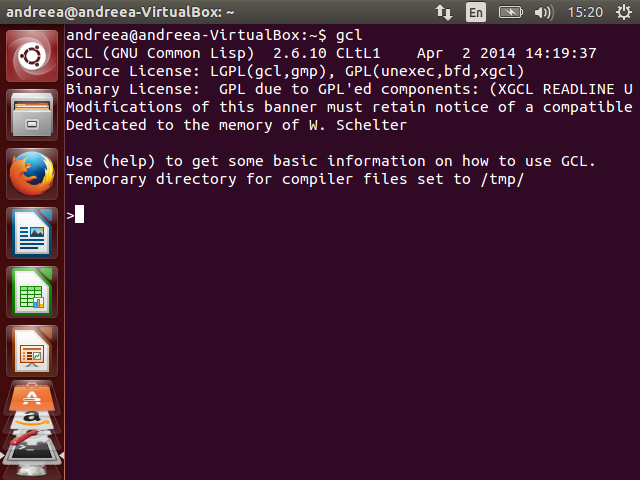
\includegraphics[width=0.7\textwidth]{fig/img5}\\
\end{figure}\\
	GCL va fi utilizat pentru implementarea si rularea unor sisteme, cat si pentru compararea diferitilor algoritmi inductive learning asupra rezultatelor obtinute de acestea. GCL va fi utilizat pentru rularea fisierelor LISP prezenta in urmatorul director: \href{http://www.cs.northwestern.edu/~paritosh/research/Bote04/v1/carve/mooney/ml-progs/}{Director fisiele LISP}. Acesta contine fisiere pentru diferiti algoritmi care folosesc acelasi format al datelor si aceeasi interfata. De asemenea, include un program pentru testarea automata utilizat pentru compararea sistemelor multiple si pentru evaluarea statistica a rezultatelor.
	Pentru a putea beneficia de aceste posibilitati, este necesara descarcarea fisierelor prezente in directorul mentionat anterior si salvarea tuturor in acelasi folder. Eu am inclus fisierele in folderul \textbf{PFOIL} aflat pe Desktop. De aceea, voi face referiri in cele ce urmeaza la calea absoluta \textbf{/home/andreea/Desktop/PFOIL}.
	Dupa ce fisierele au fost descarcate, trebuie facute unele modificari in continutul acestora pentru utilizarea acestora:
\begin{itemize}
\item Fiecare fisier ce contine instructiunea \textbf{(in-package 'user)} trebuie modificat prin comentarea acestei linii.
\item Modificarea caii absolute spre folderul ce contine fisierele cu cea a folderului creat. Acest lucru va fi realizat prin inlocuirea in fisierul "data-utilities.lisp" definirii parametrului \textbf{ml-progs-directory} la calea \textbf{"~mooney/ml-progs/"} cu cea dorita: modificarea caii absolute la \textbf{"/home/andreea/Desktop/PFOIL/"}. In imaginea ~\ref{fig:img1} este reprezentata grafica modificarea ce trebuie adusa fisierului.
\begin{figure}[h]
			\centering
			\caption{Modificare fisier "data-utilities.lisp"}
			\label{fig:img1}
			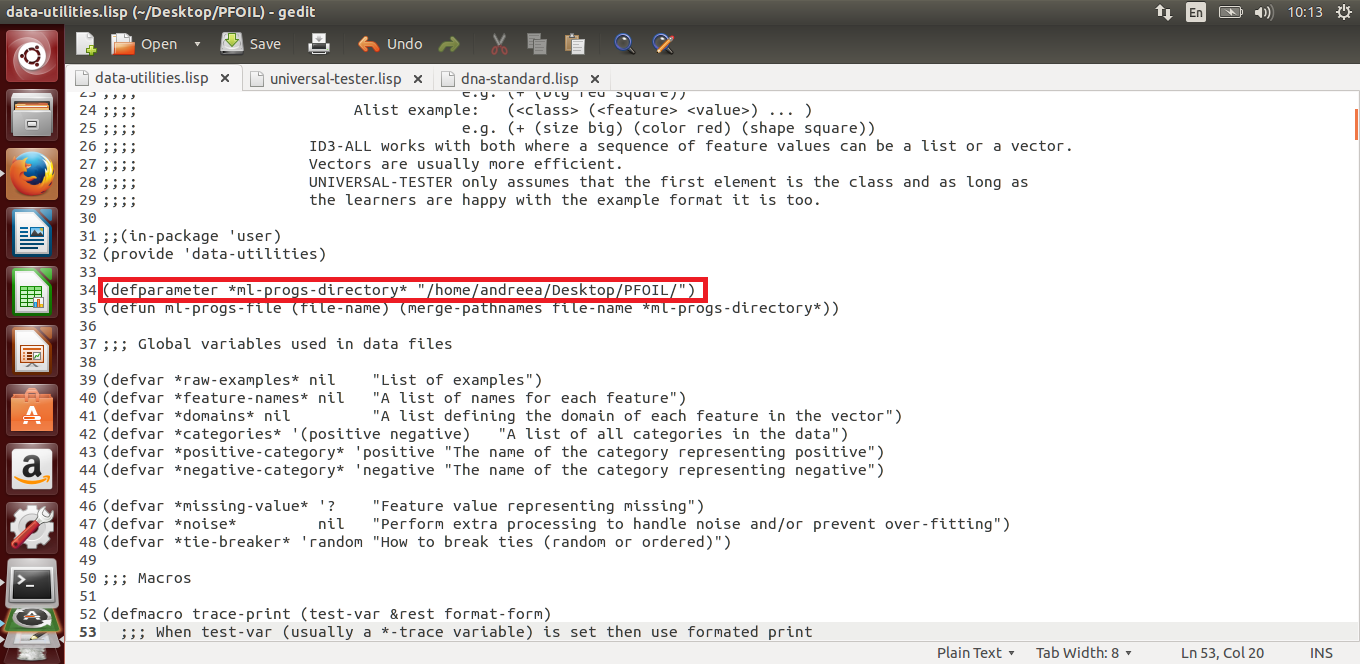
\includegraphics[width=0.7\textwidth]{fig/img1}\\
\end{figure}
\item Modificarea adusa fisierului \textbf{"universal-tester.lisp"} este urmatoarea: numele fisierelor ce vor fi atribuite modulelor \textbf{data-utilities} si \textbf{t-test} de instructiunea \textbf{require} este modificat prin adaugarea extensiei fisierelor(\textbf{.lisp}) la numele acestora.
\end{itemize}	

\section{Exercises}
\begin{enumerate}
 \item List the steps done for installing the tool. 
 \item List the exact commands needed to run the tool. 
 \item What other AI tools can use the output of your tool? 
 Can you indentify such tools on the Web?
 Try to assess the difficulty level and risks of integrating such tools for your project.
\end{enumerate}

\fbox{\begin{minipage}{16cm}
Solution to exercise 1       
\end{minipage}}
\vspace{0.5cm}

\fbox{\begin{minipage}{16cm}
Solution to exercise 2       
\end{minipage}}
\vspace{0.5cm}

\fbox{\begin{minipage}{16cm}
Epi Tools este instrumentul care se foloseste de intrari referitoare la performanta(acuratete, dimensiunea setului de date, etc) pentru a determina numarul de exemple necesare intr-un sample pentru a atinge criteriile dorite, mentionate ca si intrari. Tool-ul poate \href{http://epitools.ausvet.com.au/content.php?page=1Proportion}{Epi Tools}. 
\end{minipage}}
\vspace{0.5cm}




\chapter{Rularea si intelegerea exemplelor ($W_3$)}
	Directorul cu surse mentionat anterior contine doua seturi de date ce pot fi rulat pentru a observa functionalitatea algoritmilor de inductive learning implementati. Aceste fisiere sunt:\textit{"dna-standard.lisp"} si \textit{"labor-neg.lisp"}. 
	Fisierul \textbf{"labor-neg.lisp"} contine date necesare pentru negocierea fortei de munca in industria canadiana si fisierul \textbf{"data-standard.lisp"} contine date necesare pentru detectia cancerului prin intermediul ADN-ului.\\
	In continuare vor fi descrisi pasii necesari pentru testarea algoritmilor ID3 si PFOIL pe setul de date \textit{"dna-standard.lisp"}. Acest set contine urmatoare informatii:
\begin{itemize}
\item *FEATURE-NAMES*: o lista a numelor atributelor folosite pentru descrierea exemplelor; acest exemplu are urmatoarele atribute: P-50 P-49 P-48 P-47 P-46 P-45 P-44 P-43 P-42 P-41 P-40 P-39 P-38 P-37 P-36 P-35 P-34 P-33 P-32 P-31 P-30 P-29 P-28 P-27 P-26 P-25 P-24 P-23 P-22 P-21 P-20 P-19 P-18 P-17 P-16 P-15 P-14 P-13 P-12 P-11 P-10 P-9 P-8 P-7 P-6 P-5 P-4 P-3 P-2 P-1 P1 P2 P3 P4 P5 P6 P7;
\item *DOMAINS*: o lista ordonata cu domeniile fiecarui atribut; valorile posibile ale atributelor in acest exemplu sunt: A(adenina), G(guanina), T(timina), C(citozina).
\item *CATEGORIES*: o lista a claselor existente in setul de date; acest exemplu este clasificat in 2 clase: Promoter si Negative;
\item *THEORY*: o lista de teorii utilizata pentru deductii;
\item *raw-examples*: o lista de exemple unde primul element reprezinta clasa exemplului.
\end{itemize}
	Testarea sistemelor va fi realizata respectand urmatorii pasi:
\begin{enumerate}
\item Deschiderea terminalului si pozitionarea in folderul \textit{PFOIL} prin comanda \textbf{cd Desktop/PFOIL} introdusa in terminal.
\item Pornirea tool-ului GCL prin comanda \textbf{gcl} introdusa in terminal.
\item Introducerea comenzii \textbf{(load "universal-tester.lisp")}; aceasta comanda incarca fisierul \textit{"universal-tester.lisp"}. 
\item Introducerea comenzii \textbf{(load "id3-all.lisp")}; aceasta comanda incarca sistemul ID3 pentru inductive decision trees.
\item Introducerea comenzii \textbf{(load "pfoil.lisp")}; aceasta comanda incarca sistemul propositional FOIL pentru inductive rules.
\item Introducerea comenzii \textbf{(make-saved-tests "sample-dna-saved-tests.lisp" 10 80 '(10 25 40 80) nil "/home/andreea/Desktop/PFOIL/dna-standard.lisp")}; aceasta comanda specifica conditiile prin care va fi realizata testarea sistemului.\\
	Aceasta comanda foloseste fisierul \textit{"dna-standard.lisp"} folosit ca si set de date. Acest contine atat datele folosite pentru training, cat si cele folosite pentru testing. In comanda introdusa, valoarea \textit{80} reprezinta numarul de date folosite pentru datele de training, in timp ce valoarea \textit{nil} specifica numarul de date de testing folosite la modul default(foloseste celelalte date ramase ca si set de testing). Valoarea \textit{10} reprezinta numarul de procese ce vor fi rulate. In lista \textit{(10 25 40 80)} sunt retinute punctele folosite realizarea curbei de invatare. In fisierul \textit{"sample-dna-saved-tests.lisp"} sunt salvate informatii despre teste.
\item Introducerea comenzii \textbf{(run-saved-tests '(id3 pfoil) "sample-dna-saved-tests.lisp" "sample-dna-results")}; aceasta comanda ruleaza testele pentru compararea algoritmilor ID3 si PFOIL folosind informatiile despre teste obtinute anterior.
	In aceasta comanda \textit{sample-dna-saved-tests.lisp"} reprezinta fisierul in care sunt retinute informatiile despre teste si \textit{"sample-dna-results"}  reprezinta fisierul in care sunt salvate rezultatele testelor.
\end{enumerate}
	In urma introducerii acestor comenzi in mediul GCL, in ordinea precizata, in terminanal va fi afisat un mesaj de forma celui prezentat in imaginea ~\ref{fig:img2} in care va fi precizat timpul, complexitatea si acuratetia fiecarui algoritm utilizat dupa utilizarea unui numar de date de training din setul de date; vor fi afisate rezultatele in punctele precizate pentru realizarea curbei de invatare si operatia fi realizata de in concordanta cu numar de procese ce au fost rulate. Informatiile afisate in termina vor fi salvate si in fisierul \textit{"sample-dna-results"} sub o anumita forma, precizata in imagimea ~\ref{fig:img3}.
	
\begin{figure}[h]
			\centering
			\caption{Rezultatul testarii in terminal}
			\label{fig:img2}
			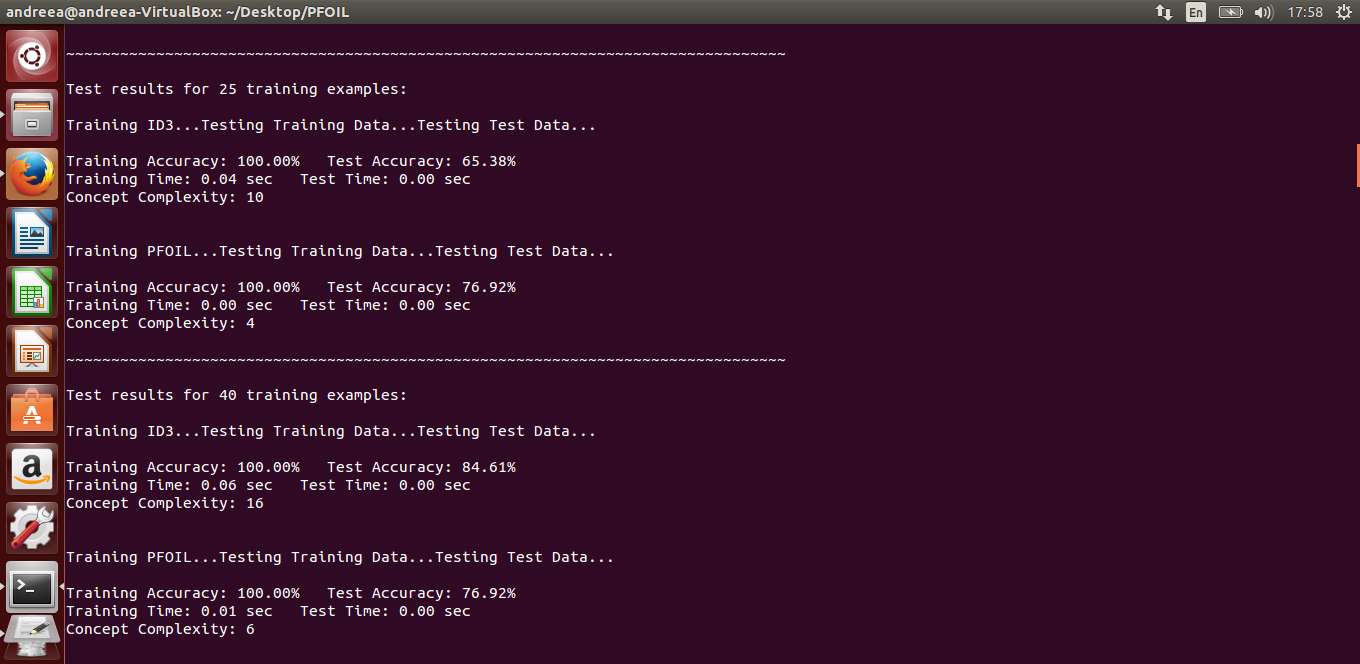
\includegraphics[width=0.7\textwidth]{fig/img2}\\
\end{figure}

\begin{figure}[h]
			\centering
			\caption{Rezultat in fisierul "sample-dna-results"}
			\label{fig:img3}
			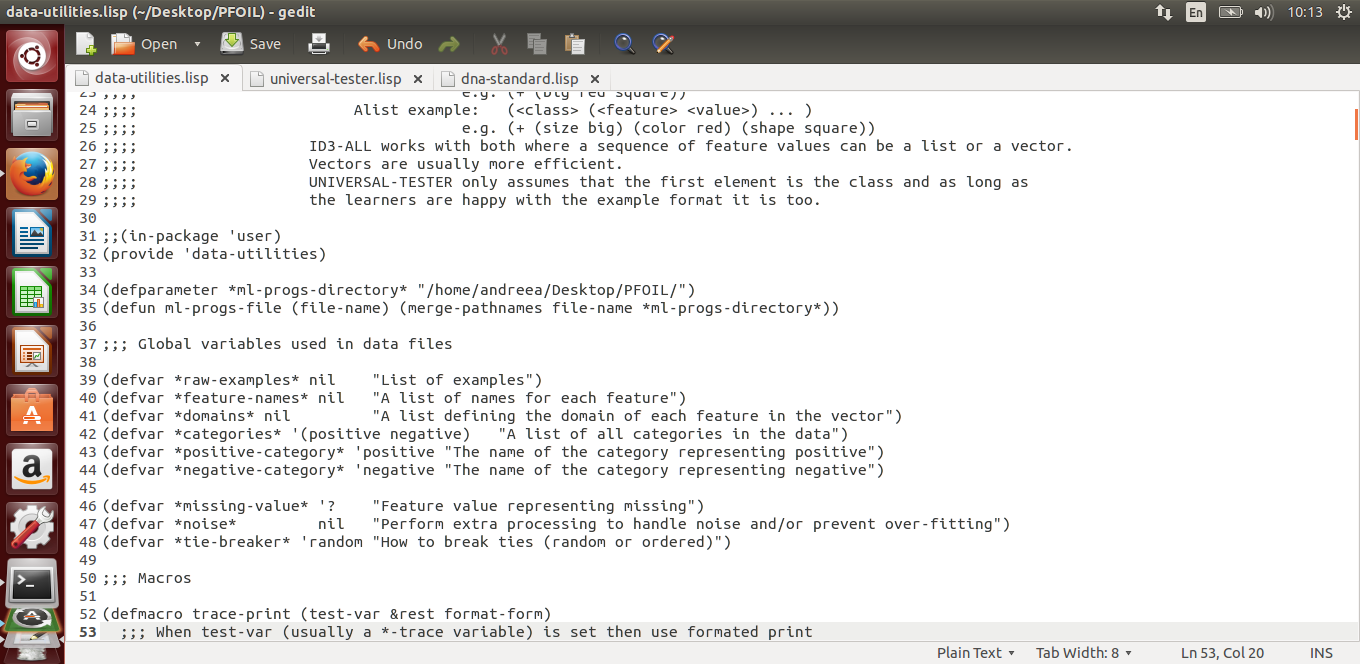
\includegraphics[width=0.7\textwidth]{fig/img3}\\
\end{figure}
	Pentru o vizualizare a rezultatelor obtinute prin testare, cu specificarea diferentelor dintre solutiile algoritmilor testati sub forma unor statistici se foloseste comanda \textbf{(t-test-file "sample-dna-results")}. Aceasta comanda compara cei doi algoritmi testati in functie de acuratetia obtinuta pe setul de testing. In imaginea ~\ref{fig:img4} este vizibil rezultatul acestei comenzi.
	
\begin{figure}[h]
			\centering
			\caption{Compararea acuratetii rezultatelor}
			\label{fig:img4}
			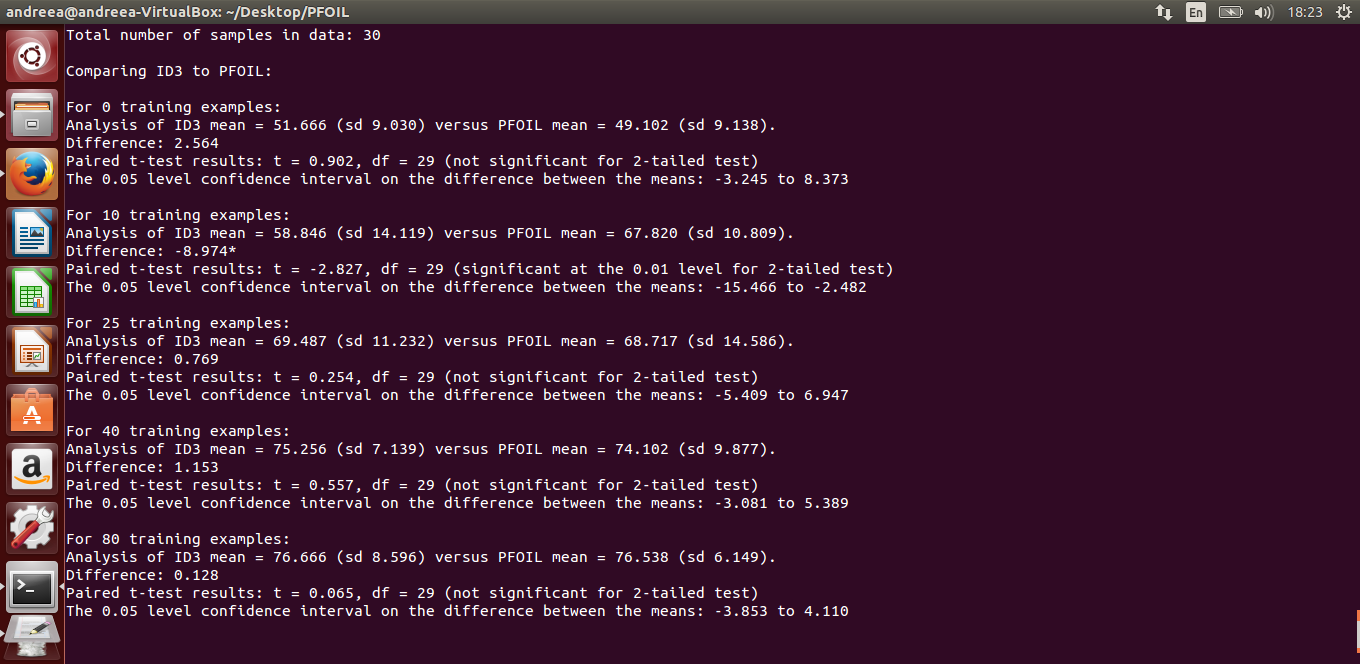
\includegraphics[width=0.7\textwidth]{fig/img4}\\
\end{figure}

\section{Exercises}
\begin{enumerate}
 \item Detail one example that you run. Which are the input and the output? 
 Describe the structure of the code. 
 \item Describe the real world problems that can be solved by your tool/algorithm.
\end{enumerate}

\fbox{\begin{minipage}{16cm}
Solution to exercise 1       
\end{minipage}}
\vspace{0.5cm}

\fbox{\begin{minipage}{16cm}
 
\end{minipage}}
\vspace{0.5cm}

 
\chapter{Intelegerea conceptelor fundamentale ($W_4$)}
	In aceasta sectiune vor fi prezentate informatii generale cu privirea la principiile ce urmeaza sa fie utilizate pentru implementarea sistemului. Realizarea acestuia se va folosi de algoritmi de Inductive learning(subdomeniul al ramurii machine learning care invata din exemple).\\
	Scopul algoritmilor Inductive learning este de a gasi o ipoteza care clasifica bine exemplele date si generalizeaza bine exemple noi. Fiecare \textbf{ipoteza} presupune ca un set de exemple sa fie clasificat ca \textbf{predicat scop}, set numit \textbf{extensie a predicatului}. Doua ipoteze cu diferite extensii sunt \textbf{inconsistente}.\\
	O ipoteza poate fi incosistenta pentru un anumit exemplu. Sunt doua cai posibile pentru ca acest lucru sa se intample:
\begin{itemize}
\item Un exemplu poate fi un exemplu \textbf{fals negativ} pentru ipoteza; acest principiu presupune ca ipoteza spune ca exemplul trebuie sa fie negativ, dar defapt el este pozitiv.
\item Un exemplu poate fi un exemplu \textbf{fals pozitiv} pentru ipoteza; acest principiu presupune ca ipoteza spune ca exemplul trebuie sa fie pozitiv, dar defapt el este negativ.
\end{itemize}
	Daca un exemplu este fals pozitiv sau fals negativ pentru o ipoteza, atunci ipoteza si exemplu sunt logic \textbf{inconsistente}. Pentru a rezolva aceasta problema, sunt realizate operatiile de \textbf{generalizare} si \textbf{specializare}. Generalizarea este utilizata in cazul intalnirii unui exemplu fals negativ si presupune adaugarea in extensia ipotezei a acestui exemplu. Specializarea este utilizata in cazul intalnirii unui exemplu fals pozitiv si presupune eliminarea din extensia ipotezei a acestui exemplu. In imaginea ~\ref{fig:img6} sunt prezentate aceste doua operatii, prin prezentarea cazurilor de ipoteza consistenta, exemplu falss negativ si exemplu fals pozitiv. 
	
\begin{figure}[h]
			\centering
			\caption{Preluata din AIMA, xapitolul 19, pg. 771}
			\label{fig:img6}
			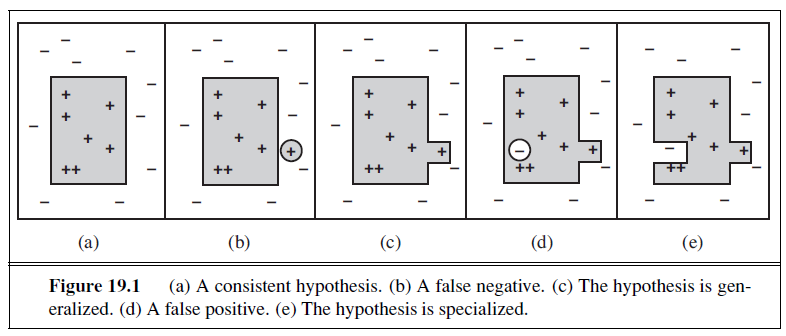
\includegraphics[width=0.7\textwidth]{fig/img6}\\
\end{figure}

	Pana acum au fost descrise principii de baza ale ramurii Inductive Learning. In continuare, vor fi prezentate conceptele fundamentale intalnite intr-o subramura a acesteia, si anume \textbf{knowledge-based inductive learning}.  Algoritmii corespunzatori acestei subramuri au urmatoarele componente:
\begin{itemize}
\item \textbf{background}: corespunde cu ipotezele initiale, care descriu cunostiinte generale despre mediul in care algoritmul este implementat;
\item \textbf{descriptions}: denota conjunctia tuturor descrierilor din setul de exemple;
\item \textbf{classifications}: denota conjunctia tuturor clasificarilor din setul de exemple;
\item \textbf{hypothesis}: corepunde cu ipotezele desprinse prin explicarea observatiilor; 
\end{itemize}
Acesti algoritmi indeplinesc urmatoarea constangere:
\begin{equation} \label{eq:1}
Background \wedge Hypothesis \wedge Descriptions \models Classifications
\end{equation}
	Ecuatia ~\ref{eq:1} prezinta ideea de baza a subramurii, prin care exemplele vor fi descrise atat de cunostiintele generale despre mediu cat si de ipoteze. La fel ca si algoritmii inductive learning, algoritmi acestei subramuri vor trebui sa gaseasca ipoteze simple consistente cu contrangerea ~\ref{eq:1}, fiind cunoscute atat descrierile si clasificarile setului de exemple, cat si cunostiintele generale. Cunostiintele despre mediul descris ajuta la gasirea unei solutii(ipoteze) mai bune si reduce spatiul de cautare a acesteia.\\
	In continuare va fi prezentata o metoda de realizare a algoritmilor Knowledge-Based Inductive Learning, metoda ce foloseste o generalizare a metodelor bazate pe arbori de decizie. Numele ei  este \textbf{Top-down inductive learning} si presupune pornirea de la ipoteza generala si specializarea acesteia in functie de setul de exemple pana la consistenta cu acesta al ipotezei. \\
	Exemplele din setul de date sunt impartite in \textit{exemple pozitive} si \textit{exemple negative}, unde clasificarea acestora este realizata in functie de conceptul ce se doreste a fi invatat prin algoritm. Metoda contruieste treptat clauze, literal cu literal, pana cand un subset din exemplele pozitive si toate exemplele negative sunt indeplinite de aceasta clauza. Acest pas continua prin adaugarea clauzei la ipoteza creata(specializare) si cu eliminarea exemplelor pozitive care sunt clasificate corect de clauza gasita anterior, dupa care procedeul este reluat pana cand setul exemplelor pozitive ce nu corespunde cu ipoteza invatate devine vid.\\
	Aceasta metoda utilizeaza o functie euristica pentru alegerea literalului ce va fi adaugat in fiecare pas al algoritmului din multimea tuturor posibililor literali ce pot fi adaugati la clauza.\\
	In continuare va fi explicat algoritmul PFOIL, algoritm din ramura Knowledge-Based Inductive Learning implementat prin metoda Top-down inductive learning, si functia euristica utilizata de acest algoritm se bazeaza pe masurarea incertitudinii reduse prin alegerea unui anumit literal.

\newpage
\begin{algorithm}
\label{alg:eval}
\caption{Algoritmul PFOIL} \label{eq:2}

\textbf{function} PFOIL($positive\ example$, $negative\ example$)\\
\KwIn{$positive\ example$ - setul de exemple pozitive\\
      $negative\ example$ - setul de exemple negative}
\KwOut{$DNF$ - ipoteza obtinuta in forma DNF}

$Pos$ $\leftarrow$ positive\ example\\
$DNF$ $\leftarrow$ \{ \}

\Do {$Pos$ este vid}{
	Fie $Neg$ setul tuturor exemplelor negative\\
	$Term$ $\leftarrow$ \{ \} \\
	$Pos2$ $\leftarrow$ $Pos$\\
	\Do {$Neg$ este vid}{
		Alege valoarea atributului care maximizeaza $DNF-gain(L, Pos2, Neg)$\\
		Adauga $L$ la termen \\
		Sterge din $Neg$ exemplele care nu satisfac $L$ \\
		Sterge din $Pos2$ toate exemplele care nu satisfac $L$
	}
	Adauga $Term$ ca un termen pentru $DNF$\\
	Sterge din $Pos$ exemplele care satisfac $Term$
}
\Return $DNF$
\newline
\newline
\textbf{function} DNF-gain(L, Pos, Neg)
	Fie $P$ numarul exemplelor din $Pos$\\
	Fie $N$ numarul exemplelor din $Neg$\\
	Fie $p$ numarul exemplelor din $Pos$ care satisfac $L$\\ 
	Fie $p$ numarul exemplelor din $Neg$ care satisfac $L$\\ 
	\Return $p*(\log_2 \frac{p}{p+n} - \log_2 \frac{P}{P+N})$

\end{algorithm}

	Algoritmul PFOIL ~\ref{eq:2} construieste o ipoteza in DNF care sa generalizeze setul de exemple pozitive si negative transmise ca si parametrii. Porneste de la setul exemplelor pozitive si adauga cate un termen in ipoteza(initial vida) pana cand setul exemplelor pozitive devine nul(ipoteza clasifica corect toate exemplele pozitive). Fiecare executie a buclei externe adauga un termen la ipoteza si elimina din setul exemplelor pozitive exemplele care sunt clasificate corect de noul termen. Fiecare executie a buclei interne adauga un literal la termenul curent folosindu-se de metrica \textbf{information gain} pentru a determina cel mai bun literal ce poate fi adaugat. Dupa alegerea literalului, exemplele negative ce nu il satisfac sunt eliminate din setul exemplelor negative(sunt negative pentru literal) si exemplele pozitive ce nu il satisfac sunt, de asemenea, eliminate din setul exemplelor pozitive(sunt negative pentru literal). Bucla interna isi termina executia la gasirea unui termen alcatuit din literali care clasifica negativ toate exemplele negative si un subset din exemplele pozitive. In acest punct, termenul este adaugat la ipoteza, setul exemplelor negative este refacut la cel initial, din setul exemplelor pozitive sunt eliminate acele exemple ce satisfac termenul curent si se reexecuta bucla interna pentru gasirea unui nou termen pe acest set de exemple pozitive.\\
	Algoritmul determina o ipoteza care generalizeaza atat setul de exemple pozitive, cat si setul de exemple negative, intrucat bucla interna se asigura ca termenul curent generalizeaza setul exemplelor negative si bucla externa se asigura ca fiecare termen adaugat va generaliza un subset din setul exemplelor pozitive pana ce toate aceste exemple vor ajunge sa fie generalizate.

\section{Exercises}
\begin{enumerate}
 \item Big O complexity
 \item Which are the latex options to write algorithms? 
 Describe in one paragraph the main features of one such package for algorithms.
\end{enumerate}

\fbox{\begin{minipage}{16cm}
Solution to exercise 1       
\end{minipage}}
\vspace{0.5cm}

\fbox{\begin{minipage}{16cm}
Solution to exercise 2       
\end{minipage}}
\vspace{0.5cm}



\chapter{Project description ($W_5$)}

The teaching objectives for this week are:
\begin{enumerate}
 \item To have a clear description of what you intend to develop.
\item To point to specific resources (datasets, knowledge bases, external tools) 
that support the development of your idea and which minimise the risk of failure.
\item To identify related work (articles) that are relevant or similar to your approach.
\end{enumerate}

\vspace{0.5cm}

My personal objectives for this class are:
\begin{enumerate}
 \item 
 \item 
\end{enumerate}


To encourage the development of AI skills, 
you  were required to come up with a significant semester project 
You have to  apply ideas from the course to a problem of your own.

Which domain to choose is a decision that only you can make. 
The more aware of the tool capabilities, the more adequate the decision.
Realistic and original scenarios are encouraged. 
Well known toy problems (salesmen, map colouring, logistic planning, wumpus, sudoku, queens, missionaries and canibals, etc.) do not worth much for your grade. 
Your scenario should be realistic and should be business oriented. 

Select clearly defined problems and not generic ones 
(i.e I will do something in the medical domain). 
Note that the focus is both on programming and on modelling the reality into a formal representation.


Before specifying your project you must understand as much as possible about the application domain (medicine, bank, human resource management, etc). 
You must also understand functionality required by the stakeholders of your system. 
Let the problem drive the modelling - the more you understand the domain, the more technical solutions need to be solved by you. 

Consider answering to the following questions:
\begin{enumerate}
 \item What will your system do?
\item Which is the scope of coverage your system aims for?
\item What will be the input of your program?
\item What will be the output of your program?
\item What will be the knowledge of your system?
\item Which would be the narrative description of running scenario(s)?
\item Which are the stakeholders of your system?
\item Which are the asumptions?
\end{enumerate}

\begin{example}[What will system do]
 
\end{example}

\begin{example}[Scope of the program]
 
\end{example}

In this problem-based model you learn what you 
need to know in order to solve a problem. 
However, note that you have total flexibility in stating your project objectives.
For instance, if you consider that studying more 
than one computational technology (or AI algorithms) brings more benefits, 
you are encourage to do it. 
You just have to frame your task under one scenario umbrella. 
One example: you can investigate the problem of {\it fake review detection} with 
various machine learning algorithms: decision trees, nayve bayes, neural networks, ensemble learning. 
This road helps you to study and compare the above algorihtms on your own problem.
A second example: you can help a {\it robot to escape from a maze} 
with various search algorithms (A*, greedy, deep first, uniform cost) 
or computation technologies (constraint satisfaction problems, planning, 
searching with observations).
Hence, both the problem-based model or a more algorithmic approach to AI 
(if formulated under the umbrella of a single scenario) 
are accepted for this laboratory.



\section{Narrative description}
This should be a simple textual description of your scenario.
You should explain your project objectives.
Put them all together in half a page.

\section{Facts}
You start the analyze of the problem by identifying 
the relevant facts from the scenario.
This fact-identification step helps you to represent the problem.


\section{Specifications}
List of specifications. 
Use your knowledge from "System Engineering" on how to write specifications and requirments (see Exercise 1).

\section{Top level design of the scenario}
Technical description of your scenario. 
In some cases, you may provide a figure with the architecture of the system. 


\section{Knowledge acquisition}
You should be aware that computing interacts with many different domains. 
Solutions to many AI problems require both computing skills and domain knowledge.

First, you should ask yourself if you have the necessary background and resources to do
a project in the chosen area. 

\paragraph{How do represent knowledge?} 
Your system relies on a knowledge base.
You have to describe how do you represent this knowledge.
You might choose between different logics: 
propositional logic, first order logic, modal logics, description logics, epistemic logics, 
temporal logics, and so on. 

\paragraph{Where are you getting the required knowledge/data}
Point towards the knowledge bases that you plan to exploit. 
The existence of these sources are required to prove that your approach is realistic.

Examples of knowledge sources include:
\begin{itemize}
\item Data sets: i.e., https://archive.ics.uci.edu/ml/datasets.html 
\item Statistics: i.e., http://ec.europa.eu/eurostat 
\item Ontology repositories in OWL or RDF format.
\end{itemize}


If you will be using books, give their reference. 
If you hope to exploit people for elicitation, give their names.
If you aim to use data sources or knowledge repositories list them and be sure that you have 
access to the needed knowledge. 
Indicate what you have accomplished so far in knowledge acquisition. 




\section{Related work}
You have to identify articles or conference papers relevant to your scenario.
Searching for adequate references can be both rewarding and frustrating.

Browse online libraries like:
\begin{itemize}
 \item Science Direct
 \item IEEE Computer Society Digital Library: IEEEXplore
 \item SpringerLink:  http://www.springerlink.com/computer-science/
 \item ACM Digital library: http://portal.acm.org/dl.cfm
%\item The Collection of Computer Science Bibliographies: http://liinwww.ira.uka.de/bibliography/
%\item Computer Science Technical Reports: http://www.nzdl.org/
\end{itemize}
A valuable resource is Google Scholar. 
Some references may be frely available on ResearchGate. 

Looking at the examples remains the best ways of learning how to present a literature analysis. 
Eacy article does include such section.


Obtain the \texttt{.bib} file of each article that you will rely on. 
Cite and very briefly describe the main idea of each paper that you have read.
Save the most relevant related papers in a local directory.
Use your own words. 
Don't use automatic translation tools (i.e., Google translate) just to expand your documentation.
You should already be aware that this is a form of cheating. 
Everything in your project that does not come with a citation is assumed to be your own work.


The following is an example of such \texttt{bib} structure:

\begin{verbatim}
 @article{bench-capon:argumentation-in-ai,
 author = {Bench-Capon, Trevor J. M.  and Dunne, Paul E. },
 title = {{A}rgumentation in {A}rtificial {I}ntelligence},
 journal = {Artificial Intelligence},
 volume = {171},
 number = {10-15},
 year = {2007},
 issn = {0004-3702},
 pages = {619--641},
 doi = {http://dx.doi.org/10.1016/j.artint.2007.05.001},
 publisher = {Elsevier Science Publishers Ltd.},
 address = {Essex, UK}
}
\end{verbatim}

Don't forget to include the above structure in your \texttt{.bib} file. 
Then, generate the \texttt{.bbl} file in order to correctly appear in the \textit{Bibliography} section.

\section{Exercises}
\begin{enumerate}
\item Sum up what is the aim of your project in a Twitter-sized phrase (140 characters)
\item Recall or identify an engineering methodology to write specifications. 
 Cite this methodology and employ it for specifying your project.
 \item Which are the differences between requirments and specifications? 
 \item Identify similar scenarios proposed by your collegues. 
 Think at some form of collaboration with one of your collegues having similar interests.
\end{enumerate}

\fbox{\begin{minipage}{16cm}
Solution to exercise 1       
\end{minipage}}
\vspace{0.5cm}

\fbox{\begin{minipage}{16cm}
Solution to exercise 2       
\end{minipage}}
\vspace{0.5cm}

\fbox{\begin{minipage}{16cm}
Solution to exercise 3       
\end{minipage}}
\vspace{0.5cm}

\fbox{\begin{minipage}{16cm}
Solution to exercise 4       
\end{minipage}}
\vspace{0.5cm}



\chapter{Preliminary results ($W_7$)}
This section corresponds to the midway report in week 7.
The teaching objectives for this week are:
\begin{enumerate}
 \item To prove that you have managed to write few lines of code of your own.
\item To prove that the knowledge or data required are already obtained.
\end{enumerate}

These objectives decreases the risk to fail. 
You should be aware that failing to meet the above objectives in week 
7 indicates high risks in obtaining relevant results at the end of the semester.
Take urgent measures to overcome these difficulties.


\section{Exercises}
\begin{enumerate}
\item Write the preliminary results explaining any realizations or insights found during the research of the subject.
\item Discuss new information and questions found during the domain investigation or during coding.
\end{enumerate}








\chapter{Implementation details ($W_9$)}

The teaching objectives for this week are:
\begin{enumerate}
 \item Illustrate each aspect of the reality that you have 
 modelled in your solution.
\item To explain the relevant code from your scenario.
\end{enumerate}

\vspace{0.5cm}

My personal objectives for this class are:
\begin{enumerate}
 \item 
 \item 
\end{enumerate}

Projects in artificial intelligence consist of developing new solutions. 


\section{Relevant code}

Provide the relevant code (see an example in Fig.~\ref{fig:code}).
You can use "verbatim" package or "listing" package. 
Complement the code with its corresponding textual description.

\begin{figure}
\begin{verbatim}
(full-reset)
(instance a Argument)
(related a b attacks)
(concept-instances Argument) 
\end{verbatim}
\caption{Modelling arguments in Racer.}
\label{fig:code} 
\end{figure}

The eager student may use concepts from \textit{literate programming}.

\section{Common bad practice in AI undergraduate projects}

\paragraph{The over-estimated AI programmer.} $ $

{\it Bad practice}: Excepting few genial students, you tend to overestimate your AI-programming abilities. 
That is, you start to write a large amount of code. (Here large might be 20 lines).
When testing it, nothing run. 
You start to debug a line or to remove it.
Your program will not run this time too. 
You remove or comment another line. 
And so on, until you have a single line of code.
If you are lucky, that could run. 
But you lose a lot of time in this enterprise.

{\it Solution}: In the early stage of writing code, write a line of code and test it. 
If it works, write another line and test it. 
And so on. 
That is, you are exploiting the interactive environments provided by 
AI tools or languages like LISP and PROLOG.
You should hold your horses and 
have the most possible skeptical attitude towards your code.  
As you get experience, your will be noticing that writing 
AI-declarative code is more effective than procedural one.  


\paragraph{The eyewash bug.} $ $
{\it Bad practice}: You spend most of your programming time to develop a GUI for your AI-system. 
Don't bother. I am sympathetic with Sania Twain's view on GUIs: "You don't impress me much".
Such things are indeed important in computer science, but not relevant in this AI class.


%\paragraph{The stucker bug} 

\paragraph{The not-organised student.}
You are not organised, if something like this will happen to you:
\begin{itemize}
 \item You do not find your project and yield "Someone removed my project!". 
Most of the time your are logged with a different user as usual. 
Check this with \texttt{who am i}. 
This is not a rhetorical question, but a Linux command.
\item You are working in a different directory. 
Type \texttt{pwd} and \texttt{ls} to check that your executables are indeed in the current working directory.
If you have been lazy to set your PATH variable, you might just forgot to type \texttt{./} 
for executing the command in the current directory.
\end{itemize}

\paragraph{The omniscient student.}
You are in this cathegory if you fail to add references. 
Reading relevant references is mandatory to deliver a decent project. 

\section{Exercises}
\begin{enumerate}
 \item What latex packages can be used to format code? 
 \item 
\end{enumerate}

\fbox{\begin{minipage}{16cm}
Solution to exercise 1       
\end{minipage}}
\vspace{0.5cm}

\fbox{\begin{minipage}{16cm}
Solution to exercise 2       
\end{minipage}}
\vspace{0.5cm}




\chapter{Tool expressivity ($W_{10}$)}


The teaching objectives for this week are:
\begin{enumerate}
 \item Describe each technical instrumentation provided 
by the tool that was enacted in your implementation.
\end{enumerate}

\vspace{0.5cm}

My personal objectives for this class are:
\begin{enumerate}
 \item 
 \item 
\end{enumerate}



%For instance:
%{\it "Racer offers also the capability to use {\it rules}. 
%he code in Fig.~\ref{fig:rules} illustrates my rule used to create instances of type student."}


\chapter{Graphs and experiments ($W_{11}$)}

The objectives for this week are:
\begin{enumerate}
 \item To describe and interpret each experiment that you have performed
\end{enumerate}

\vspace{0.5cm}

My personal objectives for this class are:
\begin{enumerate}
 \item 
 \item 
\end{enumerate}


An experiment investigates how some variables are related. 
Usually, experiments verify a previosly formulated hypothesis.
Such hypothesis may investigate how your software degrades its performance with larger inputs.
You will need to run simulations to see how your implementation is affected by different inputs.


Note that running experiments mean more than testing your solution. 
It helps to describe and prove how did you test your implementation.
Moreover, during this lab, you will often need to: 
1) generate random data for your algorithms,
2) measure their performance (number of operations, execution time),
3) draw charts,
4) interpret the obtained results.

The eager student might want to take a look at literature on how to design computer experiments, such as~\cite{fang2005design}. Section 5.6 from~\cite{fang2005design} might be of particular interest for some of you. 
If your experiments include a stochastic parameter, you need to include a test for statistical significance. 
This is important to prove that your ouputs are not a random effect.



\begin{figure}
%\includegraphics[width=8cm]{} 
Graphs always impress teachers...
\caption{Increasing the accuracy with the number of samples.}
\label{fig:accuracy}
\end{figure}

You should develop a test suite that can be used to show your code works correctly under a various conditions/problems/scenarious.


\section{Evaluation metrics}



\chapter{Related work and documentation ($W_{12}$)}

The teaching objectives for this week are:
\begin{enumerate}
 \item To compare your results to related work.
\item To discuss the advantages and limitations of your solution.
\item To deliver a professional documentation of your work.
\end{enumerate}

\vspace{0.5cm}

My personal objectives for this class are:
\begin{enumerate}
 \item 
 \item 
\end{enumerate}


This chapter convinces me that you know how your work fits into the larger domain area.


%For instance: \cite{chesnevar:Survey2000}

\section{Related approaches}
You need to support your opinions with trustworthy evidence and references.
You need also to decide how your problem fits into a wider context.
The quality of your reference is a strong indicator that you 
managed to scrutinise different perspectives on the topic.
Proving understanding of the references is the foundation of a good grade. 
By start coding without reading relevant references, you will most probable write something irelvant for the application domain.  

Identify and describe other solutions for solving the same (or similar) scenario like yours.

\section{Advantages and limitations of your solution}
This part of the conclusions chapter should be an evaluation of your work. 


\section{Possible extensions of the current work}






\chapter{Project demo and documentation ($W_{13}$)}

The teaching objectives for this week are:
\begin{enumerate}
\item Deliver the technical documentation of your project
\item Demonstrate your running scenario to the instructor
\end{enumerate}

\vspace{0.5cm}

My personal objectives for this class are:
\begin{enumerate}
 \item 
 \item 
\end{enumerate}


Demonstrate in 4-5 minutes your running scenario to the instructor. 
The demo should take place on a Linux distribution


From your final report, remove the text/examples/algorithms/rules/bibliographic references/etc - keep only your notes. 
If the documentation does not meet minimum standard for lisability and scientific discourse, 
it will be classified by the furious teaching assistant as unacceptable and therefore rejected.




\section{Exercises}
\begin{enumerate}
 \item How you would advocate your project to a possible client?
 \item Write five highlights of your results (maximum 85 characters including spaces).
 \item 
\end{enumerate}

\fbox{\begin{minipage}{16cm}
Solution to exercise 1       
\end{minipage}}
\vspace{0.5cm}

\fbox{\begin{minipage}{16cm}
Solution to exercise 2
\end{minipage}}
\vspace{0.5cm}


\chapter{Results dissemination and feedback ($W_{14}$)}

The teaching objectives for this week are:
\begin{enumerate}
\item To practice public presentation.
\item To get used with the beamer template for making scientific presentations
 \item To get feedback from your collegues. 
\end{enumerate}

\vspace{0.5cm}

My personal objectives for this class are:
\begin{enumerate}
 \item 
 \item 
\end{enumerate}

Learning is enhaced by constructive feedback on the strong/weak points of your performance during AI laboratory. 
This feedback focuses on the scientific relevance of your results and it aims to complement the feedback encapsulated in the grade.
Do not take criticism personally. 
It is the project that is being critisised, and not your competence or intelligence. 


\subsection{Public presentation}
10 slides in beamer format for a timeslot of 5 minutes presentation plus 5 minutes questions.
Questions may be posed by your collegues or the teacher. 

One of the main difficulties when designed slides is how to find the right amount of 
technical details to be included. 
No technical details rise the question of "bla bla story telling". 
To much technical details may bore the audience and also you may fail to fit within the time assigned. 

Two introductory tutorials on beamer are~\cite{mertz2005beamer} and~\cite{batts2007beamer}.
The beamer manual is: 

\href{http://cs-gw.utcluj.ro/~srazvan/articleSchema.tgz}{Presentation template}

During presentation, it is a mistake to focus on the tool that you have been used. 
During 5 minutes, you have to focus only on your results and to market your work.
Don't forget to include technical details and graphs.

A method for disseminating yor research consists of writing 3-5 highlights.
Highlights consist of a set of bullet points 
that convey the core findings of your work.
For examples, see http://www.elsevier.com/highlights.

You are now playing the role of your project advocator. 
Always keep in mind that you have to market your project only, and not the tool that you rhave relied on.



\subsection{Self-assessment}

\begin{table}
\begin{tabular}{p{8cm}l}
Aspect & Self-assessment\\ \hline
How did you manage to master the tool?& \\
How realistic was your scenario? & \\
Relevance of the running experiments &\\
Knowledge and skills achieved & \\ 
Capacity to market your effort and results through documentation and presentation& \\
\hline
\end{tabular}
\caption{Self-assessment. Assess each aspect, with: enthusiastic, satisfacatory, unsatisfacatory, bad} 
\end{table}

‘What did you do well? Give examples’

‘Where do you think the assignment is weak?’


\subsection{Formative feedback}
The last week is an opportunity for interested students to obtain 
a formative feedback. 
This is not an opportunity to negatiate your grade. 
In the previous week you had your chanches to advocate your work. 



\subsection{Problem-based learning}

One scope was to engage you in a kind of self-directed learning.
The rationale is that you are more heterogeneous and 
you have different learning experiences and maturity levels.
The focus was not on mastering AI algorithms but to apply them in practice. 
By practice I mean realistic scenarious.
Ideally, you should have developed more awareness of the social, 
environmental, economic aspects of a real problem. 


\appendix

\chapter{Your original code}
\label{app:code}
This section should contain only code developed by you, without any line re-used from other sources. 
This section helps me to correctly evaluate your amount of work and results obtained. 
Including in this section any line of code taken from someone else leads to failure of IS class this year.
Failing or forgetting to add your code in this appendix leads to grade 1.
Don't remove the above lines.




\chapter{Quick technical guide for running your project}

Requirments

Step by step technical manual

%\input{mycode}

\chapter{Check list}

\begin{enumerate}
 \item Your original code is included in the Appendix~\label{app:code}.
 \item Your original code and figures are readable.
 \item All the references are added in the Bibliography section.
  \item All your figures are referred in text (with command ref{}), described in the text, and they have relevant caption.
 \item The final documentation describes only your project. Don't forget to remove all tutorial lines in the template (like these one).
 \item The main algorithm of your tool is formalised in latex in chapter~\ref{ch:tool}.
  
\end{enumerate}


\bibliographystyle{plain}
\bibliography{is}


\vspace{2cm}
\begin{center}
Intelligent Systems Group\\

\includegraphics[width=10cm]{fig/footer}
\end{center}



\end{document}
